%!TEX root = paper.tex
\section{Discussion}
\label{sec:discussion}

\subsection{Why we think we are not missing skimmers} %{{{

Throughout the course of this study, we have been in direct communication with government officials from numerous states
responsible for the removal of skimmers, and have developed a working relationship wherein we are notified any time
a new breed of skimmer appears which is currently undetected by the Bluetana application.
%
Thus, our ability to detect skimmers depends upon the current level of investigation performed by government officials;
%
if a skimmer using a new OUI previously unflagged were to be discovered at a gas station by any of the 40+
investigators, it is likely we would be notified.
%
In fact, this has already occurred.

This lends confidence to our measurements and analysis \textit{at the current point in time}.
%
In the coming years, criminals may make a shift to using other technologies, i.e. radio, to retrieve data from
skimmers.
%
Now we will discuss ...
%}}}

\subsection{Countermeasures} %{{{

\subsubsection{EMV}
\label{sec:discussion:emv}

Credit card companies will soon require upgrading magstripe terminals to to EMV
chip technology \todo{cite}.
%
Although there are fewer vulnerabilities with EMV cards, namely the attack the
exposed reader cabling attack vector, that brought on internal skimmers
\todo{cite}.
%
There are obvious concerns on if this is realistic, as gas stations operators
were required to upgrade fuel dispensers to the new EMV-based card readers by
2018, but the deadline was extended but the large number of gas stations makes
it prohibitively expensive to do so, and therefore the deadline was extended.

Already, criminals have productised EMV versions of internal skimmers, called
deep-insert skimmers, or ``shimmers''.
%
Deep-insert skimmers bear striking resemblance to the magstripe internal
skimmers.
%
The reason is, both magstripe and chip card readers transfer card information
over a digital serial bus.
%
However, instead of tapping into the serial signal at the exposed cabling, EMV
skimmers are inserted fully into the cardslot.
%
Newer EMV chip cards obviate the need for an analog decoder by directly
providing the digital serial interface.
%
If you tap into an EMV signal you can still produce a mag-stripe card and use
it somewhere else \todo{cite}.

% \begin{figure}
% \centering
% 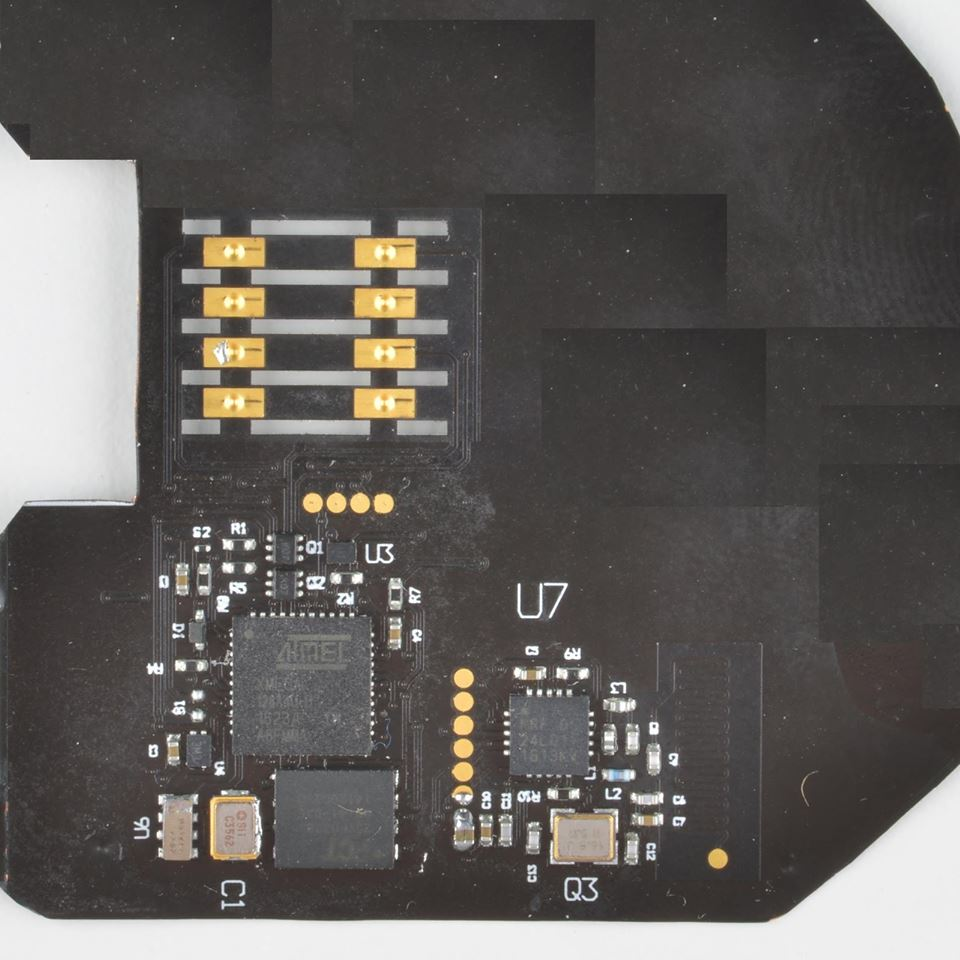
\includegraphics[width=0.5\linewidth]{fig/deep-insert}\\
% \small{Image source: gas-pump-skimmer.com}
% \caption{
% \label{fig:deep-insert}
% A ``Deep-insert'' EMV chip skimmer with wireless (Bluetooth Low-Energy) exfiltration capability.
% }
% \end{figure}

Figure~\ref{fig:deep-insert} shows an example of a deep insert skimmer that
demonstrates they are just a new version of internal skimmers in that they
passively capture card information, and they have a wireless interface for
exfiltration.

% https://link.springer.com/chapter/10.1007/978-3-642-04904-0_7
%}}}

\if 0 %{{{

\subsubsection{Physical security}
\label{sec:phys-security}

Although it would appear that card security was not a priority in the design of
fuel dispensers, the PoS circuit encrypts all payment information in transit to
the central payment processing unit in the gas station.
%
Rather, the security measures did not protect against tiny embedded system
could be installed inside the enclosure and exfiltrate the data wirelessly.
%
This is also indicated by the poor physical security in enclosure designs that
could have stopped criminals from gaining access into the internal circuitry.
%
Details about the physical security vulnerabilities of fuel dispensers are
discussed in Section~\ref{sec:phys-security}. 

\begin{figure}
\centering
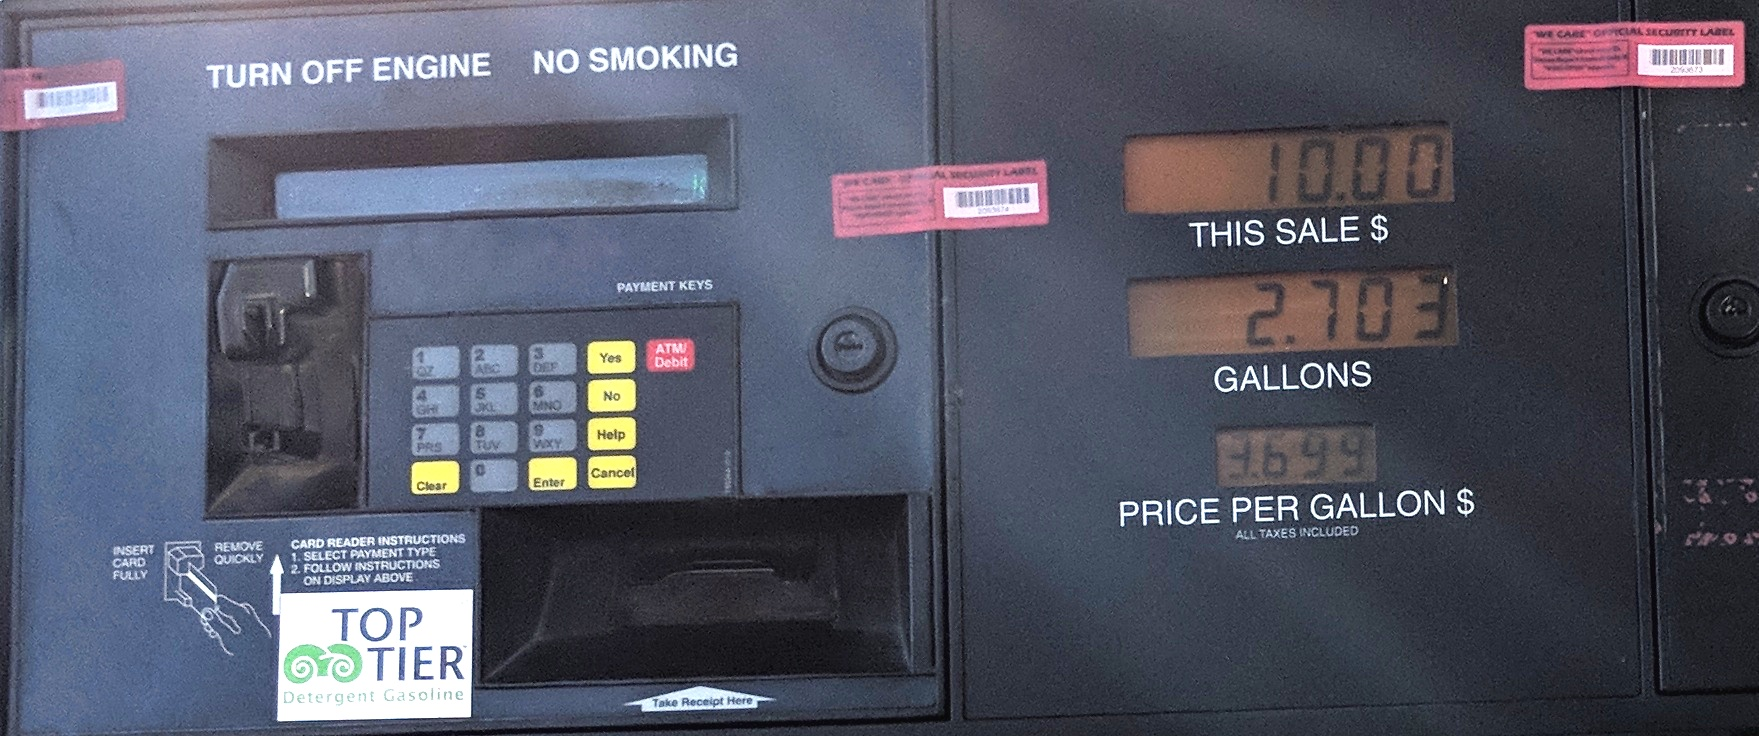
\includegraphics[width=\linewidth]{fig/tamperseal-pump.jpg}
\textbf{Multiple tamper-evident seals on a dispenser.}\\
\vspace{0.2in}
\fbox{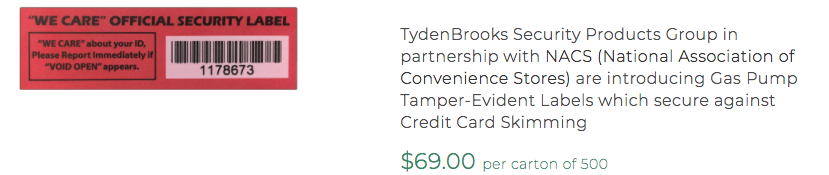
\includegraphics[width=\linewidth]{fig/tamperseal.png}}\\
\textbf{Identical seals can be purchased online.}
\caption{
\label{fig:tamperseal}
Criminals can easily replace voided seals.
}
\end{figure}

\paragraph{Tamper-evident seals}
%
Criminals also have to bypass any tamper-evident seals that the station owner
attaches to the dispensers.
%
In theory tamper-evident seals should deter criminals from installing skimmers.
%
However the significant effort required to maintain tamper-evident seals at
fuel stations makes them cumbersome to use.
%
An attendant must replace the seals every time the dispenser is inspected and
serviced.
%
Interestingly, some stations even install multiple seals with the intention of 
improving security, however this only makes it more difficult to check
if a criminal has replaced the seal with a new seal that has a different serial
number (Figure~\ref{fig:tamperseal}).
%
As such, we have found many tamper evident seals at gas stations are cut or
activated.
%
As further evidence of how ineffective security seals are, replacement security
seals were found in the possession of criminals that were arrested while they
were installing a skimmer~\cite{texas_criminal_security_seal}.





As described in the sections above, Bluetana has been and continues to be an effective weapon in the law enforcement fight against skimmers in the wild. Our methodology essentially uses characteristics of commodity Bluetooth devices in skimmers to be able to detect them. As details of our methodology become public, criminals will try to adapt to prevent skimmer detection. Based on knowledge gathered over the course of our research, in this section we try and analyze possible modifications that can be made to current skimmers to make detection more challenging, and whether Bluetana measures up. We also try to present this section as a lookahead of how the skimmer landscape might evolve in the future and thus present this as a point of reference for future work in the area.

Q : Why dont the criminals simply migrate to a longer range wireless communication mechanism like cellular?

A : By the looks of it, for a skimmer application cellular seems to be a good fit. Criminals are saved from the burden of having to drive to gas stations to collect data, thus putting more distance between them and the scene of the crime. Cellular radios however add an extra cost of requiring to purchase a SIM card with an active cellular plan. Cellular radios themselves are in general costlier than commodity Bluetooth modules and thus overall skimmer cost goes up. Addtionally, when recovered, presence of an active cellular connection can give law enforcement a much easier investigative route to pursue the criminals. Consequently, added cost and higher risk make cellular radios less likely to be used for skimmers in the future

Q : Well if not cellular, what about other wireless radios

Q : Gas pumps are now migrating to chip based readers which they are secure, so this wont be a problem in the long run, right ?

A : Not so much. Most current migration is cosmetic. Replacing entire CRIND tray mechanism or buying new machines is costly, and so current chip based modular replacements, simply read data from the cards but transmit to the backend POS in the clear. Even if we consider the case that new models of pumps based on chip readers are installed, chip based EMV mechanism has been found to be vulnerable to replay attacks because of weak RNG [cite IEEE paper]. In fact, ingenous skimmers already exist in the market that take into account these weaknesses and are able to bypass SDA, DDA and CDA to create a data dump that can be used to create perfect clones [cite website for skimmer]. However, the idea of using wireless radios to ease in the data collection and reduce chances of getting caught, are still valid and will hold. Hence focussing on this interface as a means for detection will continue to stay valid. Case in point, the chip skimmer also has a Bluetooth radio onboard

Q : A major component of your paper has been the idea of crowdsourcing, and yet you only collected data for the survey using a few individuals?

A : The idea of multiple individuals using the toolkit to detect skimmers in a large geographic area does remain valid. During development of this toolkit, we were concerned about details of our method leaking to criminals, and thus it was important to keep the circle of trusted individuals small, and thats why we the authors took to scanning the gas stations ourselves. We are in conversation with multiple state level Weights and Measures and local PDs, and will soon have large scale crowdsourcing in place. However, the fact that only a few individuals scanning for skimmers at gas stations were able to recover 10 odd skimmers, does tend to lend credence to the argument that with a large scale deployment, we will have signifantly greater capture rates

\begin{enumerate}
\item  Unnamed Devices are a limitation
\item   We use the MAC address, other metrics in that case
\item   Method in field relies more on the hitlist
\item     Hitlist can be comprehensive
\item     Using data from police recovery, as well scraping of
    websites like alibaba, sparkfun, digifruit, ebay, ...
\item    	      Incremental; if a new device shows up and
	     we are notified, we can rerun metric analysis to
	     find the new hitlist devices
\item	      method is extendable
\item What about randomized MAC addreses / smarter skimmer
\item   Full randomization, the criminal must rely on the device name
  to recover the device, since the person that is extracting the
  data is not the same as the one that implanted. Crims generally
  use mules, according to law enforcement agencies.
\item   Now, there can be a limited randomization, in which you use
  a pool of MAC addresses
\item     This is more sophisticated, and damages our methodology, the
    mitigations for this are more complicated but come in one of
    two forms: either persistent monitoring devices at each gas station
    or an even larger crowd sourced approach, wherein you get enough coverage
    of each gas station to determine persistence
\item        This is more difficult to detect. You could flag based upon whether
       the MAC address device is abnormal compared to a baseline for other
       gas stations: if you see a thermostat, it is bad.
\item        But even apple uses 47 bits of randomization, trampling upon other
       manufacturers, so how do you tell this is not another consumer
       electronic, or that the criminal is not masquerading as a common
       bluetooth device, i.e. a Tile?
\item  So consider the case of a smart criminal (i.e. one of the authors of this
paper) designing a skimmer. They would randomize the fingerprint so that
it looks like one of 255 tiles.
\item    In a largescale crowdsourced approach, you might, in the best case,
   have someone come by and scan the gas station every 3 hours. Using our
   methodology, this would not flag odd name, bad MAC, seen twice ... 
\item    There is still a possibility! For each gas station, record the geoloc
   of each of the pumps. For each gas station, check the rssi of the devices
   scanned, and see get a high confidence localization inside the pump. From
   multiple datapoints, you should be able to determine whether the bluetooth
   device is inside of a pump, and there are no bluetooth devices commonly found
   inside pumps.
\item    and you can't spoof RSSI. It is approximate, and depends on the phone/reciever
\item    Since each phone has a subjective perspective, to get the ground truth, you
   would localize to a centroid for each observer, and then combine these centroids
   to localize the skimmer.
\item    Thus, even if criminals were not dumb, we could find them.
\end{enumerate}
\fi

%}}}
